\documentclass[11pt]{article}
\usepackage[utf8]{inputenc} 
\usepackage[T1]{fontenc}
\usepackage{sectsty}
\usepackage{graphicx}
\usepackage{amsmath}
\usepackage{booktabs}
\usepackage{placeins}
\usepackage[round, authoryear]{natbib}
\usepackage[super]{nth}
\usepackage{dcolumn}
\usepackage{subcaption}
\usepackage{color} 

% Margins
\topmargin=-0.45in
\evensidemargin=0in
\oddsidemargin=0in
\textwidth=6.5in
\textheight=9.0in
\headsep=0.25in

\newcommand{\myred}[1]{\textcolor{red}{#1}}
\newcommand{\myblue}[1]{\textcolor{blue}{#1}}

\newcolumntype{d}[1]{D{.}{.}{#1}}

\begin{document}
	
\textbf{NOTE}: The contents of this file was moved to the subfile Parameterization.tex on March 19, 2022. Further edits take place in that file. 

\section{Parameterizing the model}

This section describes how we set the various parameters of the model. First, we estimate the extent to which consumers ``splurge'' when receiving an income shock. We do so using Norwegian data to be consistent with the best available evidence on the time profile of the marginal propensity to consume provided by \citet{fagereng_mpc_2021}. For this exercise we use a version of the model calibrated to the Norwegian economy. 

Second, we move on to the calibration of the full model on US data taking the splurge-factor as given. We then have different types of agents that differ according to their level of education and their subjective discount factors. Some parameters are calibrated equally for all of these different types, while some parameters are calibrated separately for each education group. Finally, a distribution of subjective discount factors is estimated separately for each education group to match features of the wealth distribution within that group. 

\subsection{Estimation of the ``splurge'' factor}
\label{sec:splurge}

We define splurging as the free spending of available income without concern for intertemporal maximization of utility. As we will show in this section, it is necessary to allow for splurging in order to capture the shorter and longer term response of consumption to income shocks. Specifically, we show that our model can account well for the results of \citet{fagereng_mpc_2021}, who study the impact of lottery winnings in Norway on consumption using millions of datapoints from the Norwegian population registry. To do so we calibrate our model to reflect the Norwegian economy and estimate the splurge factor, as well as the distribution of discount factors in the population to match two empirical moments. 

First, we take from \citet{fagereng_mpc_2021} the marginal propensity to consume out of a one-period income shock. We not only target the contemporaneous response of consumption to the income shock, but also the subsequent impact on consumption in years one through four after the shock. The share of lottery winnings expended at different time horizons, as found in \citet{fagereng_mpc_2021}, are plotted in figure \ref{fig:aggmpclotterywin}.
	
Second, we match the steady-state distribution of liquid wealth in the model to its empirical counterpart. Due to the lack of data on the liquid wealth distribution in Norway, we resort to the corresponding data from the US - assuming that liquid wealth inequality is comparable across these countries.\footnote{Data from the Norwegian tax registry contains information on liquid assets, but not liquid debt. Only total debt is reported, and this is mainly mortgage debt. Therefore, we cannot construct liquid wealth as in for example \citet{kaplan2014model}. \label{foot:liqwealth}} Specifically, we impose as targets the cumulative liquid wealth share for the entire population at the 20th, 40th, 60th and 80th income percentile, which in data from the Survey of Consumer Finance in 2004 equal $0.03$ percent, $0.35$ percent, $1.84$ percent, and $7.42$ percent.\footnote{See section~\ref{sec:SCFdata} for details.} Hence, $92.6$ percent of the total liquid wealth is held by the top income quintile. The data is plotted in figure \ref{fig:liquwealthdistribution}.

\begin{figure}[htb]
	\centering
	\begin{subfigure}[b]{.48\linewidth}
	\centering
	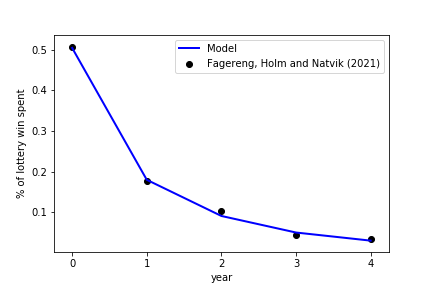
\includegraphics[width=\linewidth]{../Code/HA-Models/Target_AggMPCX_LiquWealth/Figures/AggMPC_LotteryWin}
	\caption{Share of lottery win spent}
	\label{fig:aggmpclotterywin}
	\end{subfigure}
	\begin{subfigure}[b]{.48\linewidth}
		\centering
		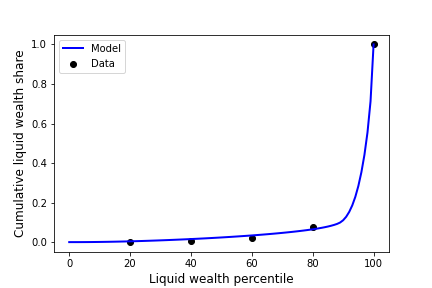
\includegraphics[width=\linewidth]{../Code/HA-Models/Target_AggMPCX_LiquWealth/Figures/LiquWealth_Distribution}
		\caption{Distribution of liquid wealth}
		\label{fig:liquwealthdistribution}
	\end{subfigure}%
	\caption{Targets and model moments from the estimation}
	\label{fig:splurge_estimation}
\end{figure}


For this estimation exercise, the remaining model parameters are calibrated to reflect the Norwegian economy. Specifically, we set the real interest rate to $2$ percent annually and the unemployment rate to $4.4$ percent, in line with \citet{aursland_state-dependent_2020}. The quarterly probability to survive is calibrated to $1-1/160$, reflecting an expected working life of 40 years. Aggregate productivity growth is set to $1$ percent annually following \citet{kravik_navigating_2019}. The unemployment net replacement rate is calibrated to $60$ percent following \citet{oecd_net_2020}. Finally, we set the real interest rate on liquid debt to $13.6$ percent and the borrowing constraint to $80$ percent of permanent income following data from the Norwegian debt registry \citet{gjeldsregistret_nokkeltall_2022}.\footnote{Specifically, we determine the average volume-weighted interest rate on liquid debt, which consists of consumer loans, credit and payment card debt and all other unsecured debt. To determine the borrowing limit on liquid debt we determine the ratio between total credit card limit divided by total wage income in Norway. We use data from December 2019. Note that although these data let us pin down aggregate quantities, they do not solve the issue referred to in footnote~\ref{foot:liqwealth}, since we cannot link them to the tax registry at the individual level.}

Estimates of the standard deviations of the permanent and transitory shocks are taken from \citet{crawley2022parsimonious} who estimate an income process on administrative data for Norwegian males from 1971 to 2014. The estimated annual variances for the permanent and transitory shocks are 0.004 and 0.033, respectively.\footnote{As shown in \citet{crawley2022parsimonious}, an income process of the form that we use here should be estimated using moments in levels not differences. Hence, we take the numbers from column 3 of their Table 4.} As in \citet{carroll2020sticky}, these are converted to quarterly values by multiplying the permanent and transitory shock variances by $1/4$ and $4$, respectively. Thus, we obtain quarterly standard deviations of $XX=0.0316$ and $XX=0.363$.

Using the calibrated model, unexpected lottery winnings are simulated and the share of the lottery spent in each year is calculated. Specifically, each simulated agent receives a lottery win in a random quarter of the first year of the simulation. The size of the lottery win is itself random and spans the range of lottery sizes found in \citet{fagereng_mpc_2021}. The estimation procedure minimizes the distance between the target and model moments by selecting the splurge factor and the distribution of discount factors in the population, where the latter are assumed to be uniformly distributed in the range $[\beta-\nabla, \beta+\nabla]$. We approximate the uniform distribution of discount factors with a discrete approximation and let the population consist of $7$ different types.

The estimation yields a splurge factor of $0.32$ and a distribution of discount factors described by $\beta = 0.986$ and a $\nabla=0.0174$. Given these estimated parameters and the remaining calibrated ones, the model is able to replicate the time path of consumption in response to a lottery win from \citet{fagereng_mpc_2021} and the targeted distribution of liquid wealth very well, see figure \ref{fig:splurge_estimation}.


\subsection{Data on permanent income, liquid wealth and education}
\label{sec:SCFdata}

Before we move on to the parameterization of the full model for the US, we describe in detail the data that we use to get measures of permanent income, liquid wealth and the division of households into educational groups. We use data on the distribution of liquid wealth from the 2004 wave of the Survey of Consumer Finance (SCF). We restrict our attention to households where the the head of the household is of working age which we define to be in the range from 25 to 62. The SCF-variable ``normal annual income'' is our measure of the household's permanent income, and to exclude outliers we drop the observations that make up the bottom 5 percent of the distribution of this variable. The smallest value of permanent income for households in our sample is thus \$16,708. 

Liquid wealth is defined as in \citet{kaplan2014model} and consists of cash, money market, checking, savings and call accounts, directly held mutual funds, stocks and bonds. We subtract off liquid debt which is the revolving debt on credit card balances. Note that the SCF does not contain information on cash holdings, so this is imputed with the procedure described in Appendix B.1 of \citet{kaplan2014model} which also describes the credit card balances that are considered part of liquid debt. We drop any households that have negative liquid wealth. 

Households are classified into three educational groups. The first group ``Dropout'' applies to households where the head of household has not obtained a high school diploma, the second group ``Highschool'' includes heads of households that have a high school diploma and those who in addition have some years of college education without obtaining a bachelor's degree, and the third group ``College'' consists of heads of households who have obtained a bachelor's degree or higher. With this classification of the education groups, the ``Dropout'' group makes up $9.3$ percent of the population, the ``Highschool'' group $52.7$ percent, and the ``College'' group $38.0$ percent. 

With our sample selection criteria we are left with a sample representing about 61.3 million US households.

\subsection{Calibrated parameters} 
\label{sec:calib}

With households divided into the three education groups, some parameters, presented in table~\ref{tab:calibAll}, are calibrated equally across all groups, while other parameters, presented in table~\ref{tab:calibEd}, are education-specific. Households are also assumed to be ex-ante heterogeneous in their subjective discount factors in addition to their level of education. 

\begin{table}[th]
\begin{center}
	\begin{tabular}{lcd{3}} 
		\toprule
		Parameter & Notation & $\text{Value}$ \\ \midrule 
		Risk aversion & & 1.0 \\ 
		Splurge & & 0.32 \\ 
		Survival probability, quarterly & & 0.994 \\
		Risk free interest rate, quarterly & & 1.01 \\ 
		Standard deviation of transitory shock & & 0.346 \\
		Standard deviation of permanent shock & & 0.0548 \\ 
		Unemployment benefits replacement rate (share of PI) & & 0.3 \\ 
		Unemployment income w/o benefits (share of PI) & & 0.05 \\ 
		Avg. duration of unemp. spell in normal times (quarters) & & 1.5 \\
		Avg. duration of unemp. benefits in normal times (quarters) & & 2 
		\\ \bottomrule 
	\end{tabular}
	\caption{Calibrated parameters that apply to all types. ``PI'' refers to permanent income.}
	\label{tab:calibAll}
\end{center}	
\end{table}

All households are assumed to have log preferences over consumption, so the coefficient of relative risk aversion is set to XX=1. We also assume that all households have the same propensity to splurge out of transitory income gains and set XX=0.32, the value estimated in section~\ref{sec:splurge}. However, each education group is divided into types that differ in their subjective discount factors. The distributions of discount factors for each education group are estimated to fit the distribution of liquid wealth within that group, and this is described in detail in section~\ref{sec:estimBetas}. Regardless of type, households face a constant survival probability each quarter. This is set to $1-1/160$, reflecting an expected working life of 40 years. The real interest rate on households' savings is set to $1$ percent annually. 

When households are born, they receive an initial level of permanent income. This initial value is drawn from a log-normal distribution which depends on the education level the household is born with. For each education group, the parameters of the distribution are determined by the mean and standard deviation of log-permanent income for households of age 25 in that education group in the SCF 2004. For the ``Dropout'' group the mean initial value of quarterly permanent income is \$6,200, for the ``Highschool'' group it is \$11,100, and for the ``College'' group it is \$14,500. The standard deviations of the log-normal distributions for each group are respectively $0.32$, $0.42$, and $0.53$. 

\begin{table}[th]
\begin{center}
	\begin{tabular}{lccc}
		\toprule 
		\multicolumn{4}{l}{Parameters calibrated for each education group} \\ 
		& Dropout & Highschool & College \\ \midrule
		Percent of population & \phantom{0}9.3 & 52.7 & 38.0 \\ 
		Avg. quarterly PI of ``newborn'' agent (\$1000) & \phantom{0}6.2 & 11.1 & 14.5 \\
		Std. dev. of $\log($PI$)$ of ``newborn'' agent & 0.32 & 0.42 & 0.53 \\
		Avg. quarterly gross growth rate of PI & 1.0036 & 1.0045 & 1.0049 \\
		Unemployment rate in normal times (percent) & \phantom{0}8.5 & \phantom{0}4.4 & \phantom{0}2.7  			
		\\ \bottomrule 
	\end{tabular}
	\caption{Parameters calibrated for each education group. ``PI'' refers to permanent income.}
	\label{tab:calibEd}
\end{center}
\end{table}

While households remain employed, their income is subject to both permanent and transitory idiosyncratic shocks. These shocks are distributed equally for the three education groups. The standard deviations of these shocks are taken from \citet{carroll2020sticky} who set the standard deviations of the transitory and permanent shocks to $XX=0.346$ and $XX=0.0548$, respectively. Permanent income also grows on average with a growth rate XX that depends on the level of education. These average growth rates are based on numbers from \citet{carroll2020modeling} who construct age-dependent expected permanent income growth factors using numbers from \citet{cagetti2003wealth} and fit the age-dependent numbers to their life-cycle model. We construct the quarterly growth rates of permanent income in our perpetual youth model by taking the average of the age-dependent growth rates during a household's working life. The average gross quarterly growth rates that we obtain for the three education groups are then $XX_d=1.0036$, $XX_h=1.0045$, and $XX_c=1.0049$.

Households also face the risk of becoming unemployed, and the parameters describing unemployment in normal times are taken from \citet{carroll2020modeling}. The unemployment benefits replacement rate is thus set to XX=0.3 for all households, and when benefits run out, the unemployment income without any benefits is set to XX=0.05. These replacement rates are set as a share of the households' permanent income. The probability of transitioning out of unemployment is also the same for all households, and is set to XX=2/3. This implies that the average duration of an unemployment spell in normal times is 1.5 quarters. The duration of unemployment benefits in normal times is set to 2 quarters. However, the different education groups do differ in the probability of transitioning into unemployment in the first place. These probabilities are set to match the average US unemployment rate by education group in 2004.\footnote{Source: Statista.com.} This average was 8.5 percent for the ``Dropout'' group, 4.4 percent for the ``Highschool'' group, and 2.7 percent for the ``College'' group. This implies that the probability of transitioning into unemployment in normal times are $XX_d=6.2$ percent, $XX_h=3.1$ percent and $XX_c=1.8$ percent. 

\subsection{Estimating the discount factor distributions} 
\label{sec:estimBetas}

Discount factor distributions are estimated separately for each education group to match the distribution of liquid wealth for households in that group. To do so, we let each education group consist of different types that differ in their subjective discount factor, $\beta$. The discount factors within each group $e\in \{d, h, c\}$ are assumed to be uniformly distributed in the range $[\beta_e-\nabla_e, \beta_e+\nabla_e]$. The parameters $\beta_e$ and $\nabla_e$ are chosen for each group separately to match the median liquid wealth to permanent income ratio and the $\nth{20}$, $\nth{40}$, $\nth{60}$, and $\nth{80}$ percentile points of the Lorenz curve for liquid wealth for that group. We approximate the uniform distribution of discount factors with a discrete approximation and let each education group consist of $7$ different types.

Panel~A of Table~\ref{tab:estimBetas} shows the estimated values of $(\beta_e, \nabla_e)$ for each education group. The panel also shows the minimum and maximum values of the discount factors we actually use in the model when we use a discrete approximation with $7$ values to the uniform distribution of discount factors. As is clear from the maximum values, all types in the model have a discount factor below $1$. 

The minimum values for the discount factors on the other hand, indicate that some of the household types in the model are very impatient, particularly in the Dropout group. This reflects that liquid wealth is very concentrated within that education group with the top quintile holding $96.4$ percent of the liquid wealth for that group. Such low estimates for discount factors are in line with those obtained in the literature on payday lending (see for example XX and XX). 

\begin{table}[th]
\begin{center}
\begin{tabular}{l}
	\begin{tabular}{lccc}
		\multicolumn{4}{l}{Panel (A) Estimated discount factor distributions} \\ 
		& Dropout & Highschool & College \\ \midrule
		$(\beta_e, \nabla_e)$ & (0.799, 0.228) & (0.937, 0.066) & (0.985,0.012) \\
		(Min, max) in approximation & (0.604, 0.995) & (0.881, 0.994) & (0.975, 0.996) \\
		\midrule 
	\end{tabular} \\ \\ 

	\begin{tabular}{lccc}
	\multicolumn{4}{l}{Panel (B) Estimation targets} \\ \midrule
	& Dropout & Highschool & College \\ \midrule
	Median LW/PI (data) & 4.64 & 30.2 & 112.8 \\ 
	Median LW/PI (model) & 4.64 & 30.2 & 112.8 \\
	 $[20,40,60,80]$ pctiles of Lorenz curve (data) & $[0, 0.01, 0.6, 3.6]$ & $[0.06, 0.6, 3.0, 11.6]$ & $[0.2, 0.9, 3.3, 10.3]$ \\
	$[20,40,60,80]$ pctiles of Lorenz curve (model) & $[0.0, 0.0, 0.5, 3.6]$ & $[0.04, 0.9, 3.7, 11.3]$ & $[0.3, 1.5, 4.0, \phantom{0}9.9]$
	\\ \midrule 
	\end{tabular} \\ \\ 

	\begin{tabular}{lcccc}
	\multicolumn{5}{l}{Panel (C) Non-targeted moments} \\ 
	& Dropout & Highschool & College & Population \\ \midrule
	Percent of total wealth (data) & 0.8 & 17.9 & 81.2 & 100 \\
	Percent of total wealth (model) & 1.6 & 21.2 & 77.3 & 100 \\
	Average quarterly MPC (model) & 0.63 & 0.38 & 0.14 & 0.31 \\
	Average annual MPC (model, incl. splurge) & 0.99 & 0.90 & 0.62 & 0.85
	\\ \bottomrule 
\end{tabular}
\end{tabular}
\caption{Estimated discount factor distributions, estimation targets and non-targeted moments.}
\label{tab:estimBetas}
\end{center}
\end{table}

Panel~B of Tabel~\ref{tab:estimBetas} and Figure~\ref{fig:LorenzPts} show the estimation targets and how well the model manages to fit them. The bottom-right quadrant of Figure~\ref{fig:LorenzPts} also shows how well the model fits the liquid wealth distribution for the population as a whole. The fit is quite close, but the model does produce a population where liquid wealth is slightly more concentrated than in the data. 

Finally, panel~C of Table~\ref{tab:estimBetas} shows that the estimated model produces a wealth distribution across the three education groups that is fairly close to the one in the data. The panel also reports the average, quarterly and annual MPCs for each education group. The quarterly MPC results from the households' decision problem where they optimally allocate between consumption and savings. The annual MPC takes into account the initial splurge factor when an income shock is first received as well as the decisions to consume  out of additional income that remains after splurging for four quarters. 

\begin{figure}[th]
	\begin{center}
	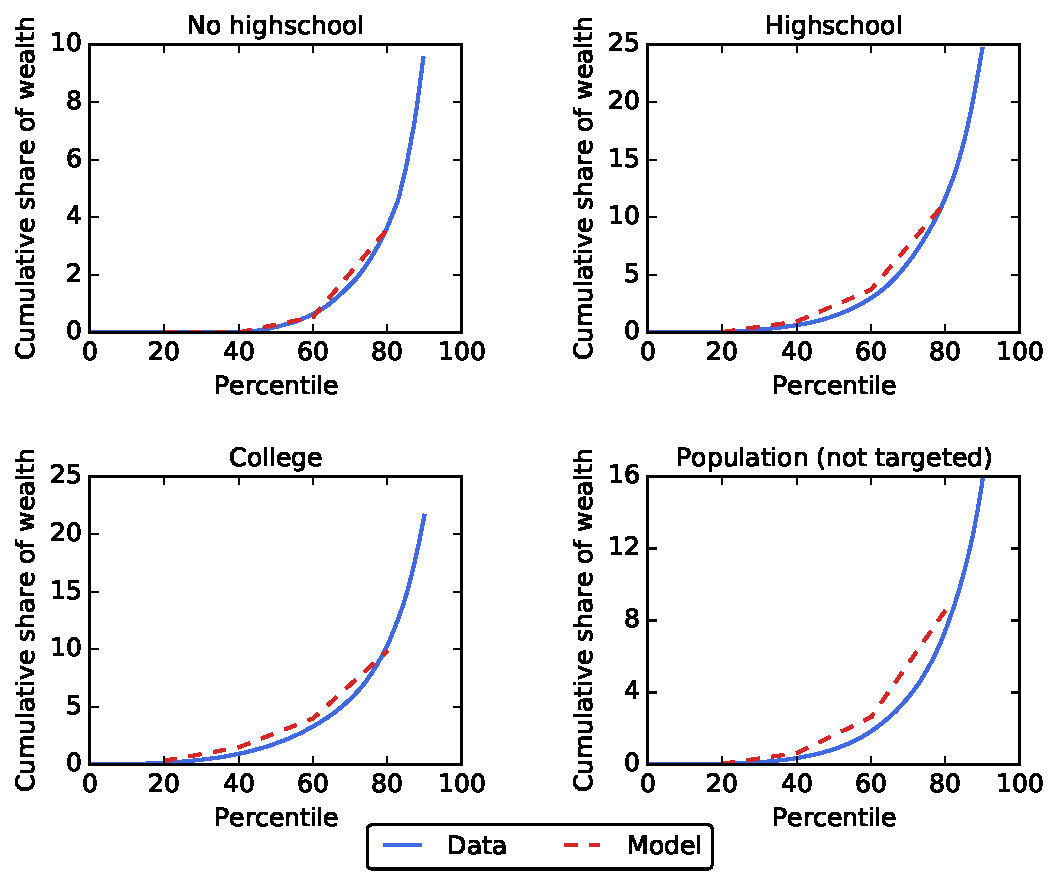
\includegraphics[width=.9\textwidth]{LorenzPoints}
	\label{fig:LorenzPts}
	\caption{Distributions of liquid wealth within each educational group and for the whole population from the 2004 Survey of Consumer Finance and from the estimated model.}
	\end{center}
\end{figure}

\let\bibfont=\small
%\bibliographystyle{econometrica}
\bibliographystyle{natbib}
\bibliography{Section_calibration_estimation}
%\pdfbookmark[1]{References}{references}

\end{document}
